\documentclass[11pt,a4paper]{article}
\usepackage[utf8]{inputenc}
\usepackage[spanish]{babel}
\usepackage{amsmath}
\usepackage{amsfonts}
\usepackage{graphicx}
\usepackage{geometry}
\usepackage{listings}
\usepackage{xcolor}
\usepackage{hyperref}

\geometry{margin=2.5cm}

% Configuración para código fuente
\definecolor{codegreen}{rgb}{0,0.6,0}
\definecolor{codegray}{rgb}{0.5,0.5,0.5}
\definecolor{codepurple}{rgb}{0.58,0,0.82}
\definecolor{backcolour}{rgb}{0.95,0.95,0.92}

\lstset{
    backgroundcolor=\color{backcolour},   
    commentstyle=\color{codegreen},
    keywordstyle=\color{magenta},
    numberstyle=\tiny\color{codegray},
    stringstyle=\color{codepurple},
    basicstyle=\ttfamily\footnotesize,
    breakatwhitespace=false,         
    breaklines=true,                 
    captionpos=b,                    
    keepspaces=true,                 
    numbers=left,                    
    numbersep=5pt,                  
    showspaces=false,                
    showstringspaces=false,
    showtabs=false,                  
    tabsize=2,
    language=Python
}

\title{\textbf{Clase Especial: Técnicas de Preparación de Datos previa a Machine Learning para Regresión}}
\author{Métodos Numéricos para Ingeniería \\ Estudiantes de 3er Semestre}
\date{\today}

\begin{document}

\maketitle

\tableofcontents
\newpage

\section{Introducción: El principio de ``Basura entra, Basura sale''}
En los modelos de regresión (como la regresión lineal o polinomial), el objetivo principal consiste en mapear una función matemática continua que minimice la distancia (o el error cuadrático) respecto a un conjunto de puntos de entrenamiento. 

Sin embargo, los algoritmos matemáticos subyacentes ---como el \textbf{Gradiente Descendente} o la \textbf{Inversión de Matrices} ($\mathbf{X}^T\mathbf{X})^{-1}$)--- son extremadamente sensibles a las perturbaciones estructurales en las variables de entrada. Si un dataset contiene escalas numéricas desproporcionadas, datos ausentes o valores atípicos severos, el espacio de búsqueda del optimizador se distorsiona, provocando inestabilidad numérica, convergencia lenta o sesgos inaceptables en los coeficientes calculados.

\section{Técnicas Principales de Preparación de Datos}

\subsection{Detección y Tratamiento de Outliers (Valores Atípicos)}
Un \textit{outlier} es una observación numérica que se desvía de forma tan extrema del resto de los datos que despierta sospechas de haber sido generada por un mecanismo o error diferente (errores de medición, fallas de sensores, etc.). En una regresión por Mínimos Cuadrados, un solo outlier con gran apalancamiento puede ``jalar'' la recta o hiperplano de regresión, sacrificando por completo el ajuste del modelo para el 99\% restante de las observaciones corporativas correctas.

Para detectarlos de manera analítica y objetiva, empleamos el \textbf{Rango Intercuartílico (IQR)}:
\begin{align}
    Q_1 &= \text{Primer Cuartil (Percentil 25)} \\
    Q_3 &= \text{Tercer Cuartil (Percentil 75)} \\
    IQR &= Q_3 - Q_1
\end{align}

Establecemos matemáticamente las fronteras de tolerancia. Cualquier dato $x$ se clasificará formalmente como outlier si cumple con el siguiente criterio de exclusión:
\begin{equation}
    x < Q_1 - 1.5 \times IQR \quad \text{ó} \quad x > Q_3 + 1.5 \times IQR
\end{equation}

\begin{figure}[h!]
    \centering
    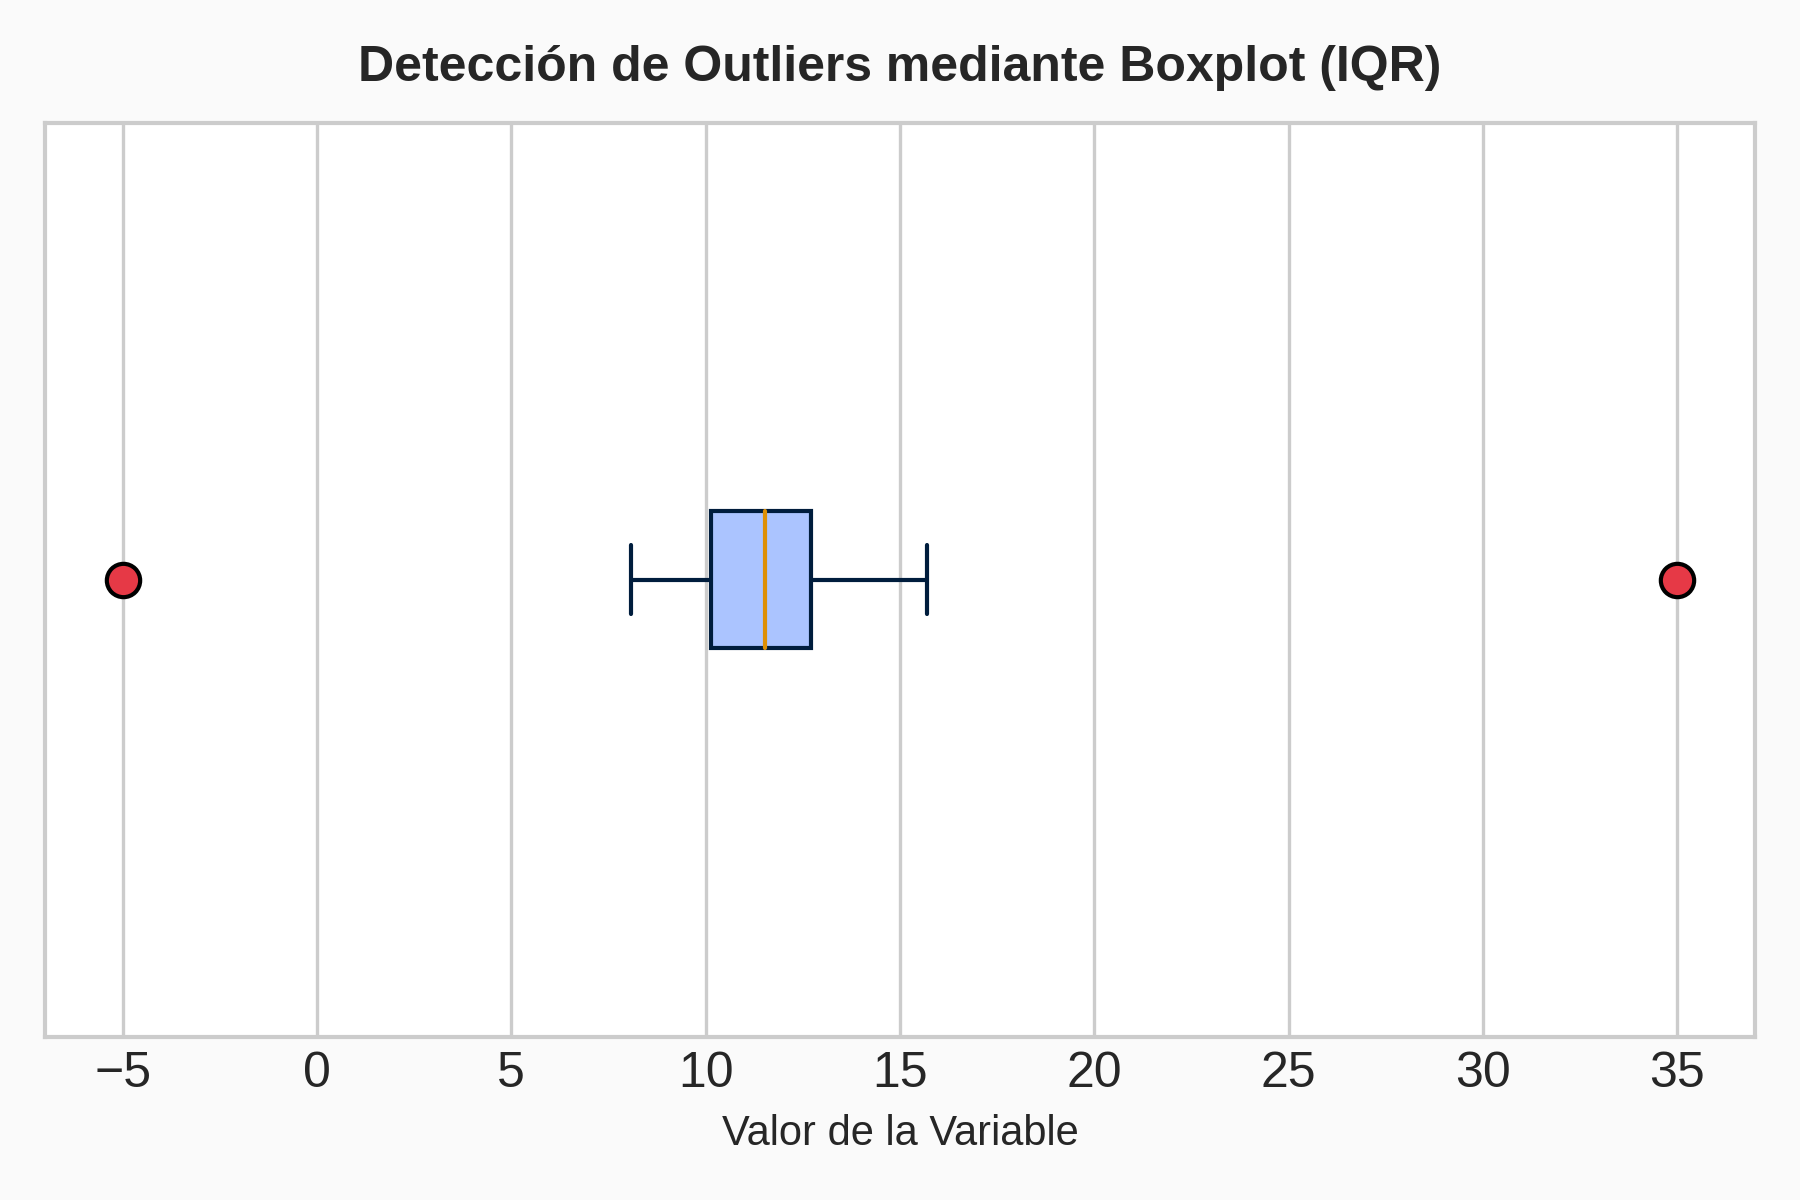
\includegraphics[width=0.65\textwidth]{images/boxplot_iqr.png}
    \caption{Identificación de valores atípicos mediante el uso de diagramas de caja (Boxplot).}
    \label{fig:boxplot}
\end{figure}

\subsection{Escalamiento Lineal (Min-Max Scaling)}
El escalamiento lineal transforma las magnitudes de una característica numérica para confinarlas de forma estricta dentro de un rango cerrado predeterminado, comúnmente $[0, 1]$. Esta técnica es fundamental cuando las variables físicas poseen dimensiones incompatibles y el algoritmo no asume distribuciones normales preestablecidas.

La fórmula de transformación aplicada a cada elemento $X$ es:
\begin{equation}
    X_{\text{scaled}} = \frac{X - X_{\min}}{X_{\max} - X_{\min}}
\end{equation}

\paragraph{Ejemplo de Ingeniería:} Considere un estudio donde se predice el precio de un bien inmobiliario basado en la \textit{Edad de la estructura} (rango de 0 a 50 años) y el \textit{Precio de mercado} (rango de 50,000 a 500,000 USD). Sin el escalamiento adecuado, el algoritmo interpretará que las variaciones en el precio son geométricamente más significativas que las variaciones de la edad, únicamente por el orden de magnitud del número bruto. Al mapear ambas dimensiones al dominio $[0,1]$, ambas variables aportan proporcionalmente al cómputo de las distancias euclidianas.

\subsection{Estandarización (Z-Score Normalization)}
La estandarización o normalización estadística transforma los datos crudos de modo que la nueva distribución resultante posea de manera exacta una \textbf{media ($\mu$) igual a 0} y una \textbf{desviación estándar ($\sigma$) igual a 1}. Es un prerrequisito mandatorio para optimizadores analíticos lineales que asumen de forma nativa que las variables de entrada se comportan bajo una distribución Gaussiana.

La ecuación de estandarización para una muestra es:
\begin{equation}
    Z = \frac{X - \mu}{\sigma}
\end{equation}

A diferencia de Min-Max, esta técnica no comprime los datos a un rango estricto, permitiendo mapear con exactitud qué tan alejado (en términos de desviaciones estándar) se encuentra un punto crítico del centro de gravedad de la población.

\section{El Concepto de Percentiles}
Para un ingeniero, comprender la posición relativa de una variable dentro de un espectro continuo es vital. Un \textbf{percentil} es una medida de posición no central que divide un conjunto de datos ordenados en 100 partes porcentualmente equivalentes. Indica el porcentaje de observaciones que son \textit{iguales o menores} que el valor evaluado.

Por ejemplo, si se determina que el tiempo de respuesta P95 (Percentil 95) de una turbina hidráulica ante una sobrecarga es de $2.1\text{ segundos}$, significa que el 95\% de todos los eventos registrados presentan un tiempo de respuesta óptimo menor o igual a $2.1\text{ segundos}$, y solo un alarmante 5\% restante supera dicho umbral crítico.

\begin{figure}[h!]
    \centering
    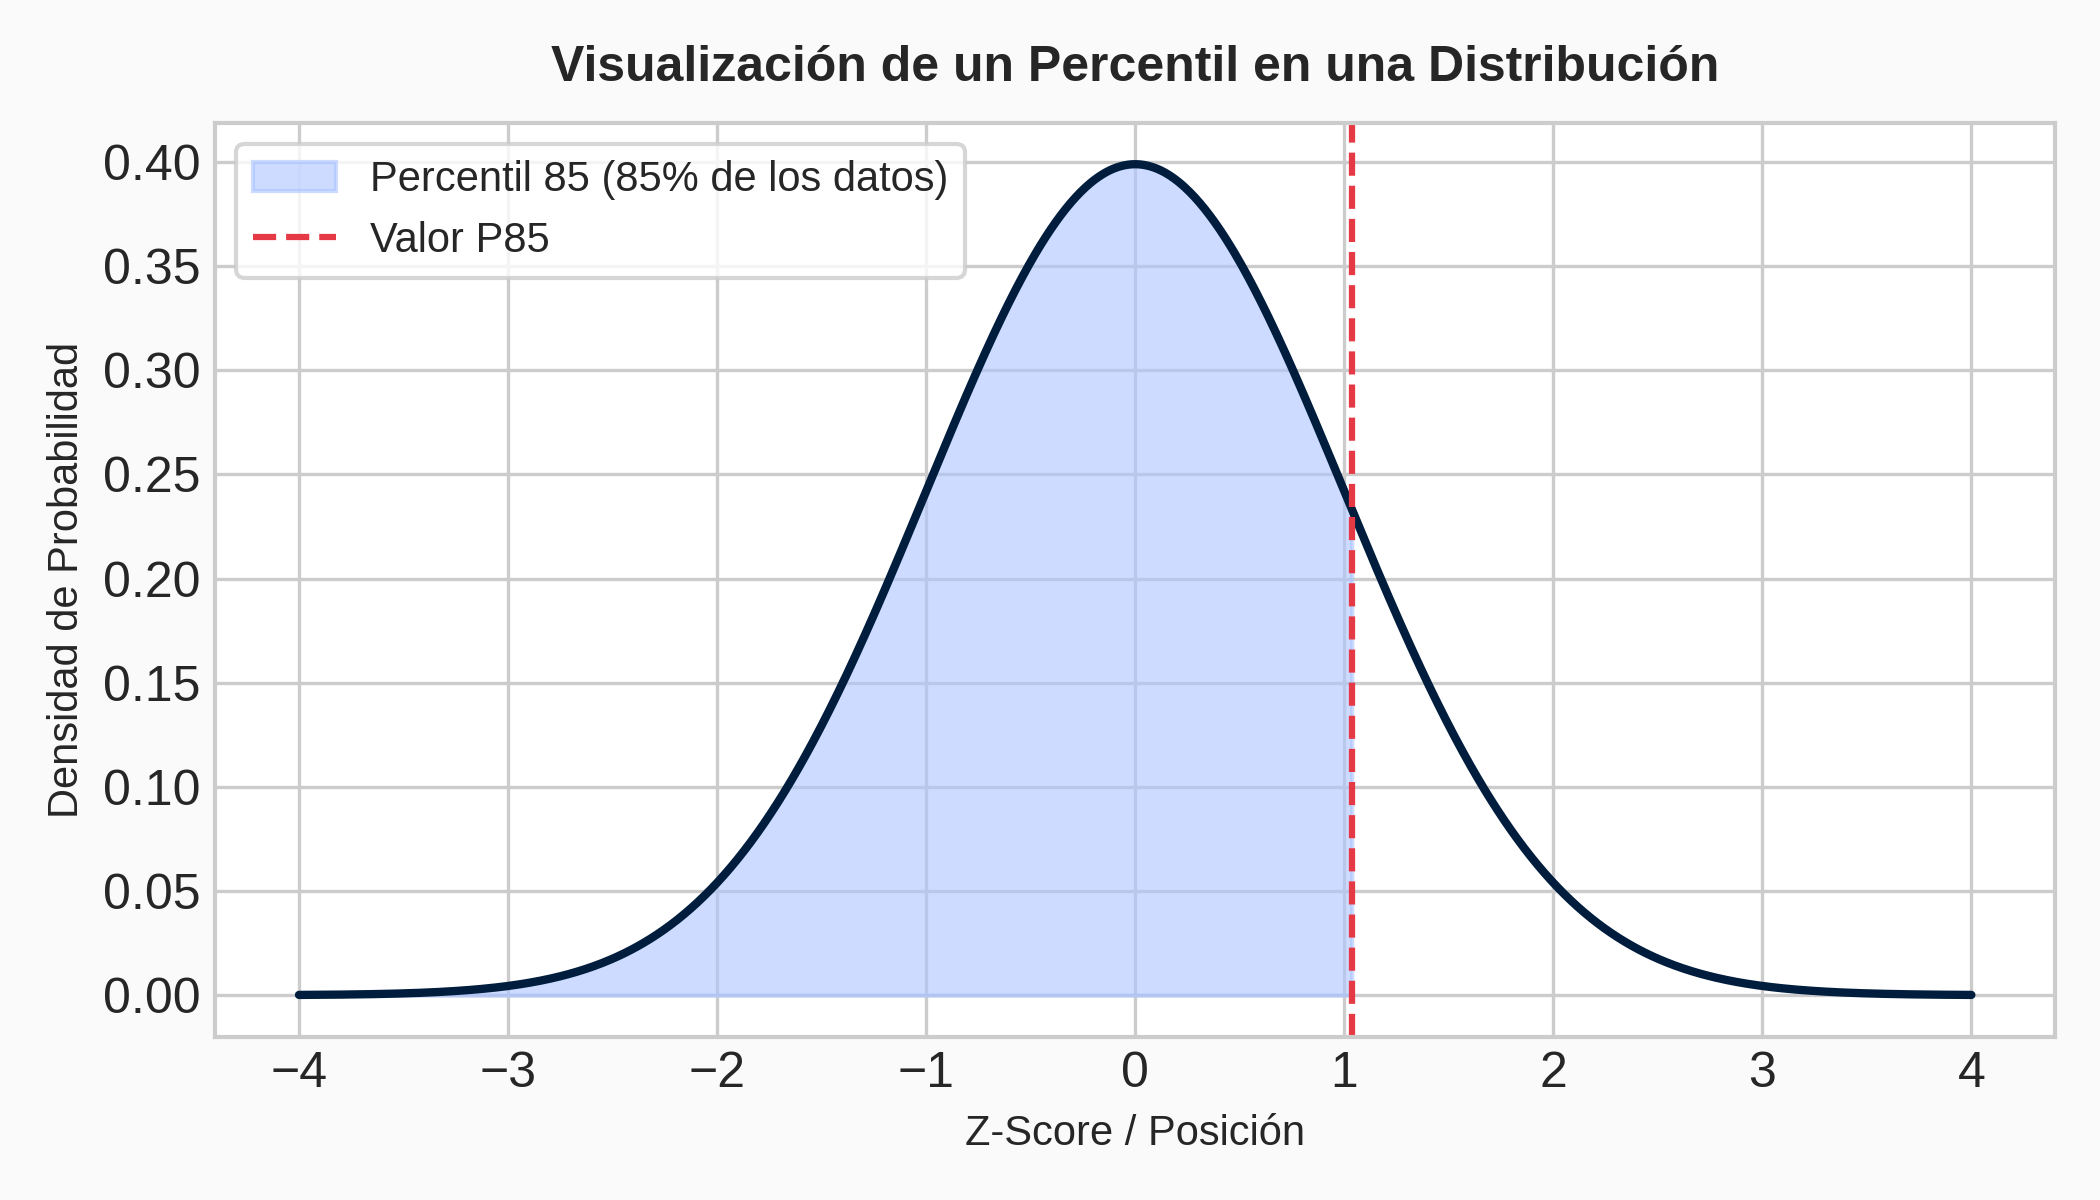
\includegraphics[width=0.7\textwidth]{images/percentiles.png}
    \caption{Representación gráfica de un percentil sobre la curva de densidad normal.}
    \label{fig:percentiles}
\end{figure}

\newpage
\section{Laboratorio Práctico en Python (Pandas y NumPy)}
A continuación, se detalla el código base implementado en la biblioteca \texttt{pandas} enfocado en la resolución de los problemas presentados en clase, asumiendo un dataset sintético sobre eficiencia energética en maquinaria pesada.

\begin{lstlisting}[language=Python, caption=Script de limpieza y transformación de variables]
import pandas as pd
import numpy as np

# 1. Construcción del dataset de simulación
data = {
    'Horas_Operacion': [10, 12, 11, 15, 9, 13, 100, 11], # El 100 es un outlier
    'RPM_Motor': [1500, 1600, 1550, 1700, 1480, 1620, 1580, 1510], # Escala macro
    'Consumo_KW': [25, 28, 26, 32, 22, 30, 29, 24]
}
df = pd.DataFrame(data)

# Tratamiento de Outliers con el método IQR
Q1 = df['Horas_Operacion'].quantile(0.25)
Q3 = df['Horas_Operacion'].quantile(0.75)
IQR = Q3 - Q1

lim_inf = Q1 - 1.5 * IQR
lim_sup = Q3 + 1.5 * IQR

df_limpio = df[(df['Horas_Operacion'] >= lim_inf) & (df['Horas_Operacion'] <= lim_sup)].copy()

# Implementación de Min-Max en RPM
min_rpm = df_limpio['RPM_Motor'].min()
max_rpm = df_limpio['RPM_Motor'].max()
df_limpio['RPM_Escalado'] = (df_limpio['RPM_Motor'] - min_rpm) / (max_rpm - min_rpm)

# Implementación de Z-Score en Horas
media_h = df_limpio['Horas_Operacion'].mean()
std_h = df_limpio['Horas_Operacion'].std()
df_limpio['Horas_Estandarizado'] = (df_limpio['Horas_Operacion'] - media_h) / std_h

print(df_limpio)
\end{lstlisting}

\section{Lista de Verificación (Checklist) para el Estudiante}
\begin{enumerate}
    \item \textbf{Exploración Inicial:} Verificar simetría y detectar valores atípicos severos mediante el método analítico IQR.
    \item \textbf{Tratamiento previo:} Decidir remoción o imputación antes de alterar las escalas corporativas globales.
    \item \textbf{Selección de Escala:} 
    \begin{itemize}
        \item Usar \textbf{Z-Score} si el algoritmo subyacente asume distribuciones gaussianas o requiere estabilidad en la media (p. ej., Regresiones Lineales con penalización Ridge/Lasso).
        \item Usar \textbf{Min-Max} si el algoritmo requiere límites acotados estrictos sin suposiciones probabilísticas (p. ej., Redes Neuronales Artificiales).
    \end{itemize}
\end{enumerate}

\end{document}
